%
%	design.tex
%
%	Final Report: Design
%
%	John Hughes and Michael Jean
%	University of Manitoba
%

\chapter{Design}
\label{ch:design}

The overall end goal of this project is to develop 4 electronic modules for the 2010 Formula SAE vehicle, as described before. The discussion of design in this chapter will also include information about the larger systems that each module is a part of in order to provide context. The mechanical portions of the design will be discussed in less detail than the electrical systems, since this is the focus of this thesis.

The architecture can be divided into 4 distinct systems that communicate over a shared network. These systems are:

\begin{itemize}
\item the \emph{engine} system;
\item the \emph{braking} system;
\item the \emph{wireless telemetry} system; and
\item the \emph{driver interface} system.
\end{itemize}

\section{Common Design Features}
\label{sec:common_design_features}

\nomenclature{PCB}{Printed Circuit Board}

At the heart of each system is a module that controls all aspects of the system's function, or compliments existing functionality. Each module is implemented on a custom \emph{Printed Circuit Board} (PCB) with an \emph{AT90CAN128} micro-controller from Atmel. All software is written in C and uploaded through a standard IEEE 1149.1 JTAG interface. Each module has common {}``life-support'' systems such as a voltage regulator and decoupling capacitors. A specialized 23-pin header is attached to the PCB to connect it to the inter-module network, the power supply, and whatever systems it needs to interact with.

\section{Inter-module Communication}
\label{sec:inter_module_communication}

\nomenclature{CAN}{Controller Area Network}

All electronic systems on the vehicle communicate over a two-wire \emph{Controller Area Network} (CAN) bus operating at 1 MBit/s. Every system module has a Microchip-brand MCP2551 CAN transceiver IC for connecting their local micro-controller to the bus, and all modules are capable of being a termination point for the bus.

\begin{table}[H]
	\caption{Common module components.}
	\label{table:common_module_components}
	\centering
	\begin{tabular}{|c|c|c|}
		\hline 
		Part & Manufacturer & Part Number\tabularnewline 
		\hline \hline
		CAN Bus Transceiver & Microchip & MCP2551\tabularnewline \hline
		Microcontroller & Atmel & AT90CAN128\tabularnewline \hline
		Voltage Regulator & Linear Technology & LT1129CST5\tabularnewline		
		\hline
	\end{tabular}
\end{table}

Testing system functionality requires a means of injecting messages onto the CAN bus that links the various modules together. To facilitate this, a \emph{network testing} module was developed. This module allows us to interface directly with individual nodes on the network, and to test parts of the system independently of one another. 

The network tester consists of an off-the-shelf AT90CAN128 development board from Olimex, and custom software. The PC-interfaceable network tester runs a set of test suites. Each test suite will test all functions of a given module by sending and receiving the expected messages on the network to the module. This allowed us to test and debug each module independently as well as the entire network together.

%
% Engine System
%

\section{Engine System}
\label{sec:engine_system}

The engine system consists of:

\begin{itemize}
\item the \emph{transmission} sub-system, for shifting gears;
\item the \emph{starter} sub-system, for starting the motor from dead stop; 
\item the \emph{intake management} sub-system, for controlling the length of the intake runners; and
\item the \emph{engine module}, which controls the sub-systems.
\end{itemize}

The three sub-systems consist of a network of electromechanical actuators, sensors, and electronics. The \emph{engine module} acts as the control centre for the engine system. This design pattern is common throughout the other vehicle systems, as will be demonstrated in later sections.

\begin{figure}[H]
	\centering
		\begin{tikzpicture}[auto, node distance=2.5cm, draw=black!70, >=stealth']
  \node [bus, name=can1] {};
  \node [bus, name=can2, below of=can1] {};
  \node [bus, name=can3, below of=can2] {};
  \node [bus, name=can4, below of=can3, above=1cm] {};

  \draw [-, line width=2pt] (can1) -- (can2);
  \draw [-, line width=2pt] (can2) -- node[rotate=90, above] {CAN Bus} (can3);
  \draw [-, line width=2pt] (can3) -- (can4);

  \node [bus, above of=can1, below=1cm] (tip1) {};
  \node [bus, below of=can4, above=1cm] (tip2) {};
  \draw [-, densely dashed, line width=2pt] (can1) -- (tip1);
  \draw [-, densely dashed, line width=2pt] (can4) -- (tip2);

  \node [block, right of=can2, right, text width=8em] (engine) {Engine Module};
  \node [block, right of=can3, right, text width=8em] (ecu) {ECU};

  \node [block, right of=engine, right, text width=8em] (starter) {Starter System};
  \node [block, right of=ecu, right, text width=8em] (intake) {Intake System};
  \node [block, above of=starter, text width=8em] (transmission) {Transmission System};

  \draw [<->] (engine) -- (ecu);
  \draw [<->] (engine.south east) -- (intake.north west);
  \draw [<->] (engine) -- (starter);
  \draw [<->] (engine.north east) -- (transmission.south west);

  \draw [<->, line width=2pt] (can2) -- (engine);
  \draw [<->, line width=2pt] (can3) -- (ecu);
\end{tikzpicture}
	\caption{Engine system overview.}
	\label{fig:engine_system_overview}
\end{figure}

\subsection{Transmission System}

In Section \ref{sec:transmission_control_background} the background of the transmission and the control system used in previous years was discussed. The design of the transmission control scheme for this project therefore improves upon the previous generation by targetting several of the noted deficiencies, while reusing specific portions that worked well.

The decision was made to continue to use pneumatic actuators, although extensive research was made into the possibility of using electric actuators with gearboxes. It was determined that a far greater force-to-weight ratio could be achieved with the pneumatic actuators in comparison with the electric, as well as significant cost savings.

\subsubsection{Pneumatics}

After deciding to not change away from pneumatics, an improved actuation scheme was proposed that would both improve the controllability and efficiency of the system. A diagram of the mechanical portion of the pneumatics system can be seen in Figure \ref{fig:pneumatics}. An on-board compressed air tank is fitted with a pressure regulator, which regulates the system pressure to approximately $120\,psi$. 4 electronically controlled pneumatic valves control the flow of air to and from 2 pneumatic actuators.

\paragraph{Shift Actuator}

The first actuator, visible on the left of Figure \ref{fig:pneumatics}, actuates the shift lever between 3 different positions: upshift, downshift, and rest-state. The transmission spring-loads the lever to automatically return to the rest-state, which we have set up to be half-way through the actuator stroke. Individually applying pressure to one port will pull the lever up, and to the other port, down.



\begin{figure}
  \centering
  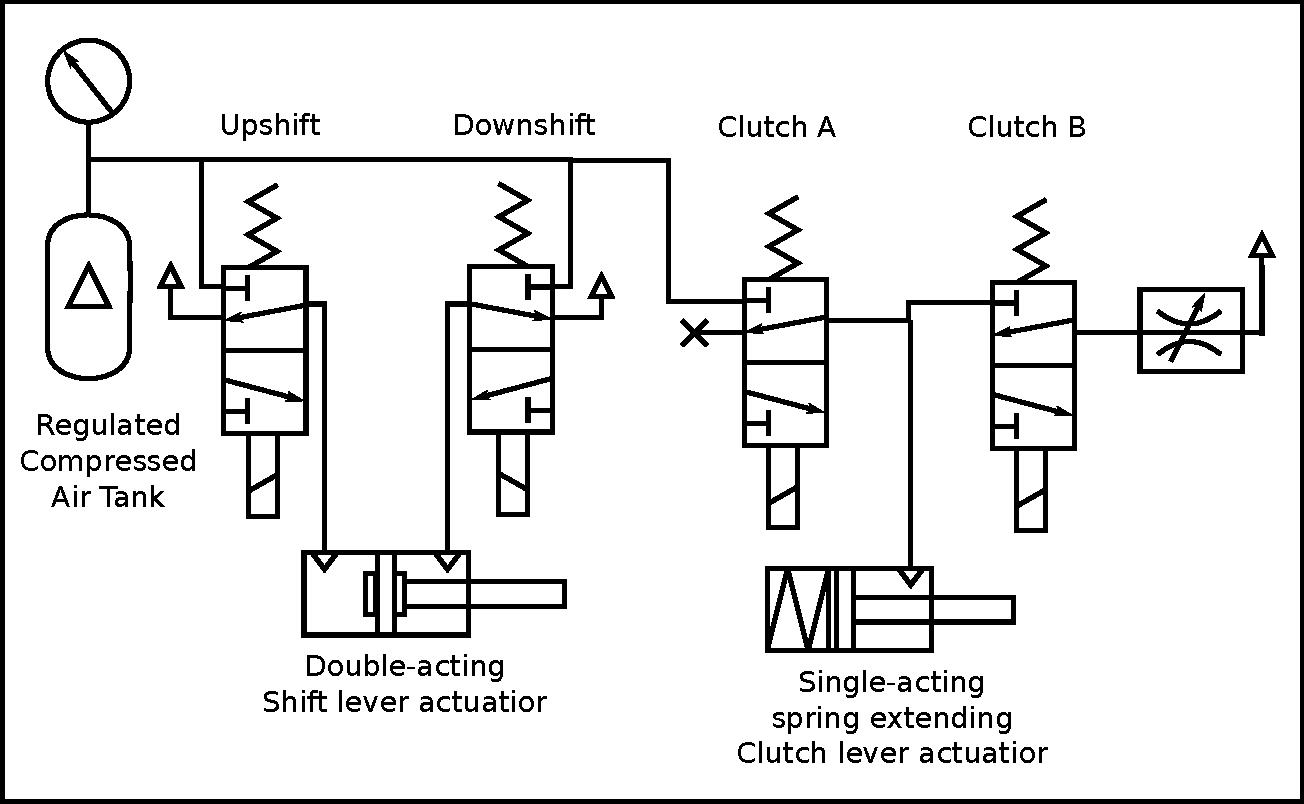
\includegraphics[scale=0.5]{Figures/pneumatics.pdf}
  \caption{Transmission control pneumatics design.}
  \label{fig:pneumatics}
\end{figure}

The 2010 transmission control system further de-tasks the driver, improves shift performance, and improves accuracy by providing precise positioning of the clutch lever. This precision in control allows for a {}``partial-throttle launch'' without a hand-lever, and results in less mechanical strain on the clutch and transmission. 

\nomenclature{PWM}{Pulse Width Modulation}

Precise control of the clutch lever is accomplished with a fast solenoid valve controlled by a closed loop feedback system. The fast solenoid valves are controlled with \emph{Pulse Width Modulation} (PWM), which allows precise control of the air flow into the cylinder. Position feedback for the clutch and gear levers is provided by rotary potentiometers. Current gear position is determined with a potentiometer that is mechanically linked to the shift drum. Control and timing are generated by the micro-controller.

The shift lever does not require the same level of control as the clutch, but utilizes the same hardware to facilitate the possibility of using a stock shifting drum without gear position feedback.

\begin{figure}[H]
	\centering
		\begin{tikzpicture} [auto, node distance=2cm, draw=black!70, >=stealth', text width=1cm, minimum width=1.5cm]
  \node [module, minimum width=12cm, text width=5cm] (engine) {Engine Module};

  \node [small block] at ($(engine.south east)!0.1!(engine.south west)+(0,-1.5cm)$) (clutch_valve) {Clutch Valve};
  \node [small block] at ($(engine.south east)!0.5!(engine.south west)+(0,-1.5cm)$) (shift_valve) {Shift Valve};
  \node [small block] at ($(engine.south east)!0.9!(engine.south west)+(0,-1.5cm)$) (gear_pot) {Gear Pot};

  \node [small block, text width=1.5cm, below of=clutch_valve] (clutch_cylinder) {Clutch Cylinder};
  \node [small block, below of=clutch_cylinder] (clutch_lever) {Clutch Lever};
  \node [small block, text width=1.5cm, left of=clutch_cylinder, left=-0.25cm] (position_sensor) {Position Sensor};
  \node [small block, text width=1.5cm, below of=shift_valve] (shift_cylinder) {Shift Cylinder};
  \node [small block, below of=shift_cylinder] (shift_lever) {Shift Lever};
  \node [small block, text width=1.5cm, left of=shift_cylinder, left=-0.25cm] (position_sensor2) {Position Sensor};
  \node [small block, below of=gear_pot] (shift_drum) {Shift Drum};

  \draw [->] ($(engine.south east)!0.1!(engine.south west)$) -- (clutch_valve);
  \draw [->, dashed] (clutch_valve) -- (clutch_cylinder);
  \draw [->, dashed] (clutch_cylinder) -- (position_sensor);
  \draw [->, dashed] (clutch_cylinder) -- (clutch_lever);
  \draw [->] (position_sensor) -- ($(engine.south east)!0.1!(engine.south west)+(-2.70cm,0)$);

  \draw [->] ($(engine.south east)!0.5!(engine.south west)$) -- (shift_valve);
  \draw [->, dashed] (shift_valve) -- (shift_cylinder);
  \draw [->, dashed] (shift_cylinder) -- (shift_lever);
  \draw [->, dashed] (shift_cylinder) -- (position_sensor2);
  \draw [->] (position_sensor2) -- ($(engine.south east)!0.5!(engine.south west)+(-2.70cm,0)$);

  \draw [<-] ($(engine.south east)!0.9!(engine.south west)$) -- (gear_pot);
  \draw [<-, dashed] (gear_pot) -- (shift_drum);
\end{tikzpicture}
	\caption{Transmission system overview.}
	\label{fig:transmission_system_overview}
\end{figure}

Sizeable consideration was made for replacing the pneumatic system with a fully electronic one. However, it was determined that the power to weight ratio of electric motors and gearboxes was far less than that of a pneumatic solution for the amount of torque required.

\subsection{Starter System}

The starter solenoid is energized by signals from the engine controller. The driver may choose between an \emph{automatic} or \emph{manual} starting sequence. The \emph{driver interface module} (described in section \ref{sec:driver_interface_system}) relays the particular starting sequence command to the engine controller through the CAN bus.

\begin{figure}[H]
	\centering
		\begin{tikzpicture}[auto, node distance=2cm, draw=black!70, >=stealth']
  \node [block] (engine) {Engine Module};
  \node [block, right of=engine, right] (starter) {Starter Solenoid};
  \node [block, right of=starter, right] (motor) {Starter Motor};
  \node [block, right of=motor, right] (ice) {ICE};

  \draw [->] (engine) -- (starter);
  \draw [->] (starter) -- (motor);
  \draw [->, dashed] (motor) -- (ice);
\end{tikzpicture}
	\caption{Starter system overview.}
	\label{fig:starter_system_overview}
\end{figure}

The \emph{automatic} starting sequence powers the starter solenoid until either the engine starts or a timeout elapses. In this case, the timeout is five seconds. The \emph{manual} starting sequence will engage the starter for as long as the driver demands, much like holding the key in the start position in a standard consumer automobile ignition system. 

The starter feature is disabled while the engine is running to avoid damaging the vehicle. The engine state can be determined by monitoring the current RPM.

\subsection{Intake Management System}

As mentioned in section \ref{sec:ice_overview}, much research has been put into the concept of a variable intake plenum. Engineers typically design the intake length to be optimal for torque at one specific RPM. We utilize an intake system which allows for the length of runners to be dynamically changed at runtime. The intake runners will be lengthened or shortened at different RPM values. This will serve to widen the torque response of the engine over a larger range of RPMs. A servo mechanism actuates a two-position variable intake plenum. As engine RPM changes, the servo is actuated accordingly to maximize torque output.

\begin{figure}[H]
	\centering
		\begin{tikzpicture}[auto, node distance=2cm, draw=black!70, >=stealth']
  \node [block] (engine) {Engine Module};
  \node [block, right of=engine, right] (servo) {Intake Servo};
  \node [block, right of=servo, right] (plenum) {Variable Intake Plenum};

  \draw [->] (engine) -- (servo);
  \draw [->, dashed] (servo) -- (plenum);
\end{tikzpicture}
	\caption{Intake system overview.}
	\label{fig:intake_system_overview}
\end{figure}

\subsection{Engine Module}
\label{sec:engine_module}

The \emph{engine module} is implemented on a custom PCB with an \emph{AT90CAN128} micro-controller from Atmel. All software for the micro-controller is written in C and uploaded through a standard IEEE 1149.1 JTAG interface. The module is linked to the other system modules with a CAN bus. All inter-module communication is done over the CAN bus.

In addition to the common life-support hardware for the micro-controller (such as the voltage regulator and decoupling capacitors), the engine module includes an SPI capable octal \emph{low-side solenoid driver}. This driver chip switches the low side of the solenoid valves, as well as the starter solenoid. It includes flyback protection circuitry to squash voltage spikes from the inductive load of the solenoid, and can also detect electrical shorts. 

\begin{table}[H]
	\caption{Engine module components.}
	\label{table:engine_module_components}
	\centering
	\begin{tabular}{|c|c|c|}
		\hline 
		Part & Manufacturer & Part Number\tabularnewline 
		\hline \hline
		Solenoid Driver & ST Microelectronics & L9822E\tabularnewline \hline
		\hline
	\end{tabular}
\end{table}

Besides controlling the transmission, starter, and intake management sub-systems, the engine controller software implements several driver control features:

\begin{description}

\item[Auto Upshift Feature]

This feature of the engine module is aimed primarily at improving performance in the acceleration event. Based on known torque curves, a table of optimal shift points in the RPM range is developed. As the engine reaches the top RPM for a given gear, the engine module will automatically upshift to the next gear, without any driver input. All the driver needs to do is maintain full throttle, and hold on.

\item[Full-Throttle Launch]
Full-throttle launch uses an important feature of the ECU called launch control. From a stand-still, the slip ratio of the driven wheels to the non-driven wheels is monitored, and the engine output power is reduced until the ratio reaches 1:1. Drivers use this feature by maintaining full-throttle at the starting line while holding the brake pedal. As soon as the brake pedal is released, the the engine module will release the clutch in a controlled manner in an attempt to get the best possible acceleration.

\item[Part-Throttle Launch]
Part-throttle launch is a feature designed to mimic an automatic transmission. By controlling the clutch position, and thereby modulating the amount of torque transferred to the wheels for a short period of time, the car can be made to creep slowly from a standstill. This will be used when driving up to the starting line of various dynamic events.

\item[Neutral Find]
As drivers come in to the pits from driving the course, a useful feature is the ability for the car to shift the transmission back into neutral to avoid stalling the car. The neutral find feature will automatically downshift the transmission repeatedly until it finds neutral.

\end{description}

%
% Brake System
%

\section{Brake System}
\label{brake_system}

Electronic control of the brake bias is realized with the \emph{brake system}. Drivers may adjust the brake bias from cockpit controls, allowing different drivers to {}``dial-in'' their preferred bias setting. Brake pressure is also monitored and communicated to the other modules.

The brake system consists of: 

\begin{itemize}
\item the \emph{adjustment motor}, for moving the adjusting shaft;
\item the \emph{end-of-travel sensors}, for calibrating the system; 
\item the \emph{pressure sensors}, for monitoring the state of the brakign system; and
\item the \emph{brake module}, which controls the adjustment process.
\end{itemize}

\subsection{Adjustment Motor}

A low-torque, bipolar permanent magnet stepper motor will be mechanically coupled to the bar, so that it may move with the adjustment shaft, and travel vertically when the pedal is pressed. Little torque is required to rotate the adjustment shaft, so no motor gearing is required. 

\subsection{End-of-Travel Sensors}

Automatic calibration is enabled by sensing the furthest extents in both directions of the bias bar. Microswitches will signal the brake module when the bar has reached an outer limit. 

\subsection{Pressure Sensors}

Both the front and rear brake systems have their own pressure sensors, which read the pressure in each system and translate them into a voltage for sampling by the brake module. The extents of the brake pressures for each system (i.e., brakes fully released and brakes fully applied) must be calibrated.

\subsection{Brake Module}

The brake module is implemented on a custom PCB with the same AT90CAN128 micro-controller common to the other modules. In addition to the common life-support hardware, the brake module includes a stepper motor driver to generate the complex output signals required to drive the stepper motor.

\subsection{Bias Bar Calibration Sequence}

The current bias position will be saved in non-volatile memory inside the micro-controller, so that calibration is not necessary on start-up. Occasionally, the system may be calibrated by signalling the brake module to begin it's calibration sequence over the CAN bus. During calibration, the bar will move from it's furthest extents and count the number of steps required. It will then move to the centre position.

\subsection{Pressure Calibration Sequence}

Both the fully-applied and fully-released pressures for the front and rear systems are saved inside non-volatile memory. Occasionally, these pressures should be re-calibrated. A simple procedure to calibrate the systems may be initiated by the driver. This procedure involves:

\begin{enumerate}
\item Releasing the brakes and indicating they are released; and
\item Fully applying the brakes and indicating they are applied.
\end{enumerate}

Once completed, the pressure ranges for each system are saved and the module can judge if the brakes are applied.

%
% Wireless Telemetry
%

\section{Wireless Telemetry System}
\label{wireless_telemetry_system}

The ability to communicate with the car wirelessly is a very important feature of most current FSAE designs. The ECU and DAQ provide sensor information that must be accessed wirelessly. Both provide a wired RS-232 serial interface to a Windows PC running proprietary software that communicates with each device. Each program expects to talk directly to the device through a Windows COM port. Background information on the ECU's digital interfaces is described in Section \ref{sec:ecu_data}.

The \emph{wireless telemetry system} provides a means for multiplexing these data streams and sending them wirelessly to laptops. The vehicle-side of the telemetry system consists of:

\begin{itemize}
\item the \emph{telemetry module}, which gathers and multiplexes the data; and
\item the \emph{wireless transmitter}, which modulates and transmits RS-232 over wireless to a receiver.
\end{itemize}

The remote-side of the telemetry system consists of a wireless receiver, which demodulates the RS-232 signal and directs it to the correct application.

\subsection{Telemetry Module}

The telemetry module is implemented on a custom PCB with the same AT90CAN128 micro-controller common to the other modules. In addition to the common life-support hardware, the telemetry module includes a dual RS-232 transceiver chip and two DE-9 connectors. 

The ECU and the DAQ connect to the telemetry board with specialized cables that connect to the wiring harness. The ECU and DAQ interface with two built-in USART ports on the micro-controller. A third, SPI-based UART interfaces with the wireless transmitter. 

\subsection{Wireless Transmitter}

The wireless transmitter is an XBee Pro Modem from Digi International. The modem is in a package designed for mounting on a printed circuit board, and is attached to the telemetry module directly. This modems requires a 3.3V power supply. and consumes at most 215mA of current during transmit. Since the common module hardware only provides power for 5V devices, the telemetry module has a second LDO regulator providing 3.3V. A separate antenna port is connected to the modem and mounted in the side of the module enclosure.

\subsection{Wireless Receiver}

The wireless receiver is another XBee Pro Modem with a USB interface for connecting to a laptop. The XBee packets are directed to two virtual COM ports.

  \begin{figure}[H]
    \centering
      \def\antenna{
  -- +(0mm,4.0mm) -- +(2.625mm,7.5mm) -- +(-2.625mm,7.5mm) -- +(0mm,4.0mm)
}

\begin{tikzpicture}[auto, node distance=4cm, draw=black!70, >=stealth']
  \node [block, name=max3100] {Max3100 SPI UART};
  \node [block, name=at90, right of=max3100] {AT90CAN};
  \node [block, name=rs232, right of=at90] {Max232 RS232 Transceiver};
  
  \node [block, name=can, below of=at90, above=1cm] {MCP2551 CAN Transceiver};
  \node [block, name=modem, left of=can] {XBee Modem};
  
  \node [block, name=ecu, right of=rs232] {ECU};
  \node [block, name=dac, below of=ecu, above=1cm] {DAC};

  \path (at90.north)+(0.0,+0.4) node (title) {Telemetry Module};

   \begin{pgfonlayer}{background}
       \path (max3100.north west)+(-0.3,0.7) node (a) {};
       \path (can.south -| rs232.east)+(+0.3,-0.2) node (b) {};
       \path[module] (a) rectangle (b);
   \end{pgfonlayer}

  \node [bus, name=can1, below of=can, label=below:CAN Bus, above=2.5cm] {CAN Bus};
  \node [bus, name=can2, left of=can1] {};
  \node [bus, name=can3, right of=can1] {};

  \draw [-, thick] (modem.west) -| ($(modem.west)+(-0.8,0.2)$) \antenna;

  \draw [-, line width=3pt] (can) -- (can1);
  \draw [-, line width=3pt] (can1) -- (can2);
  \draw [-, line width=3pt] (can1) -- (can3);

  \draw [<->, thick] (at90) -- node[] {SPI} (max3100);
  \draw [<->, thick] (max3100) -- node[text width=2cm] {Serial} (modem);
  \draw [<->, thick] ($(at90.east)+(0,0.1)$) to[myncbar, arm=1cm] ($(rs232.north west)+(0,-0.5)$);
  \draw [<-, thick] ($(at90.east)+(0,-0.1)$) to[myncbar, arm=1cm] ($(rs232.south west)+(0,+0.5)$);

  \draw [<->, thick] ($(rs232.north east)+(0,-0.5)$) to[myncbar, arm=1cm] (ecu);
  \draw [<-, thick] ($(rs232.south east)+(0,0.5)$) to[myncbar, arm=1cm] (dac);

  \draw [<->, thick] (at90) -- (can);

%  \draw [<->, thick] (modem) -- node[] {} (telemetry);
%  \draw [<->, thick] (telemetry) -- node[] {RS232} (ecu);
%  \draw [<->, thick] (telemetry) -- node[] {RS232} (daq);
%  \draw [-, thick] (modem) -- node[text width=1.5cm] {} (ant) \antenna;
\end{tikzpicture}
    \caption{Block Diagram, Wireless Telemetry Module.\label{fig:tele_tx_overview}}
  \end{figure}

  \begin{figure}[H]
    \centering
      \def\antenna{
  -- +(0mm,4.0mm) -- +(2.625mm,7.5mm) -- +(-2.625mm,7.5mm) -- +(0mm,4.0mm)
}

\begin{tikzpicture}[auto, node distance=3cm, draw=black!70, >=stealth']
  \node [block, name=modem] {XBee Modem};
  \node [block, name=laptop, below of=modem] {Laptop};
  \node [block, name=ecu, left of=laptop, left=0.5cm] {ECU Software};
  \node [block, name=daq, right of=laptop, right=0.5cm] {DAQ Software};
  \node [bus, name=ant, above of=modem, below=1.5cm] {};

  \draw [<->, thick] (modem) -- node[] {} (laptop);
  \draw [<->, thick] (laptop) -- node[] {RS232} (ecu);
  \draw [<->, thick] (laptop) -- node[] {RS232} (daq);
  \draw [-, thick] (modem) -- node[text width=1.5cm] {} (ant) \antenna;
\end{tikzpicture}
    \caption{The wireless telemetry system, receiver side.\label{fig:tele_rx_overview}}
  \end{figure}

  \begin{table}[H]
    \caption{Wireless Telemetry Module Components\label{tab:Wireless-Telemetry-Module}}
    \centering
      \begin{tabular}{|c|c|c|}
	\hline 
	Part & Manufacturer & Part Number\tabularnewline
	\hline
	\hline
	XBee-PRO OEM Module & Digi International & XBee-PRO\tabularnewline
	\hline 
	Dual RS232 Transceiver & Maxim Electronics & MAX232\tabularnewline
	\hline 
	SPI-capable UART chip & Maxim Electronics & MAX3100\tabularnewline
	\hline 
	300mA Low Dropout Regulator & Linear Technology & LT1521\tabularnewline
	\hline
      \end{tabular}
  \end{table}

%
%	Driver Interface System
%

\section{Driver Interface System}
\label{sec:driver_interface_system}

\nomenclature{LCD}{Liquid Crystal Display}

In previous years, the team has often been hindered by a lack of direct information from the electronic systems in the car. The driver interface module remedies this by providing information to the driver in real-time, and allows the driver to control aspects of the electronic control systems.

The driver interface system consists of:

\begin{itemize}
\item \emph{driver controls}, which are tactile inputs for adjusting vehicle dynamics; 
\item the \emph{information display panel}, which displays vehicle information to the driver; and
\item the \emph{driver interface module} which collects information from the driver controls and other modules in the system and relays them to the driver through the information display panel, and also relays driver inputs to the other modules.
\end{itemize}

\begin{table}[H]
	\caption{Driver interface components.}
	\label{table:driver_interface_components}
	\centering
	\begin{tabular}{|c|c|c|}
		\hline 
		Part & Manufacturer & Part Number\tabularnewline
		\hline
		\hline 
		Monochrome Transflective LCD & Newhaven & NHD-320240WX\tabularnewline
		\hline 
		Dot Matrix LCD Controller & RAiO & RA8835\tabularnewline
		\hline 
		ECW detented Rotary Encoder & Bourns Inc. & ECW1J-B24-BC0024L-ND\tabularnewline
		\hline
	\end{tabular}
\end{table}

\subsection{Vehicle Dynamics Mode (VDM)}
\nomenclature{VDM}{Vehicle Dynamics Mode}

The driver interface system provides a method of quickly modifying several dynamic vehicle parameters quickly and easily. For example, an acceleration event calls for launch control, auto-upshift, and a heavy forward brake bias. It is possible to enable all of these features in one step by changing the VDM mode to {}``acceleration''. 

When a new mode is selected, all nodes on the network are notified and synchronized to modify their dynamic parameters in accordance with the specific mode. For example, when the  {}``acceleration'' mode is enabled, the engine module will enable launch control and auto-upshift, and the brake controller will modify the brake bias to a pre-set ratio.

\begin{description}
  \item [{Pit Mode}] enables soft-launch driving characteristics that mimic a fully automatic transmission. This makes slowly driving the car forward from a stand-still far easier, and only requires the driver to take their left foot off the brake, and slightly apply the throttle.
  \item [{Acceleration Mode}] puts the vehicle systems into full-performance characteristics. Launch control is activated. The engine module will watch for a launch signal from the driver, and will automatically up-shift based on the engine RPM.
  \item [{Dynamic Mode}] puts the vehicle systems into a mode that is suitable for the autocross, and the endurance race.
\end{description}

\subsection{Driver Controls}

The driver controls consist of three rotary encoder knobs and three buttons. See table \ref{table:driver_controls} for a description of each.

\begin{table}[H]
	\caption{Available driver controls.\label{table:driver_controls}}
	\centering
	\begin{tabular}{|c|c|p{8 cm}|}
		\hline 
		Type & Name & Description \\
		\hline
		\hline 
		Rotary & VDM & Changes the current VDM setting. \\
		\hline 
		Rotary & Option & Changes the currently selected menu option. \\
		\hline
		Rotary & Adjust & Adjusts the value associated with the currently selected menu option. \\
		\hline
		Button & Starter & Engages the automatic start sequence if pressed once, or the manual start sequence if held down.\\
		\hline
		Button & Neutral Find & Activates the neutral-find feature. \\
		\hline
		Button & Diagnostics/Save & Pages through diagnostic information if pressed once, or saves the current dynamic settings to the selected VDM if held down.\\		
		\hline 		
	\end{tabular}
\end{table}

\begin{description}
	\item[VDM] 

\end{description}

The driver may use the \emph{Option} knob to select various vehicle dynamics to adjust. Once the desired option is selected, the \emph{Adjust} knob can be rotated to adjust the dynamic. The driver may hold the \emph{Save} button to overwrite the current VDM settings with the newly entered parameters. 

\subsection{Information Display Panel}

The interface display panel is a large monochrome \emph{Liquid Crystal Display} (LCD) screen, inset into the steering wheel. The panel provides real-time information to the driver regarding all of the electronic systems in the car. The LCD is an off the shelf module, complete with controller, character RAM, and drivers. It will provide an 8-bit parallel interface to the micro-controller. 

Primary information displayed on the panel includes:

\begin{itemize}
\item the selected gear;
\item the active \emph{vehicle dynamics mode} (VDM);
\item the telemetry signal strength;
\item the engine RPM;
\item the vehicle wheel speed; and
\item the status of the launch control feature.
\end{itemize}

The list of available options and the current value for the selected option is displayed on screen when the driver rotates the option dial. After a timeout period, normal real-time information display resumes. 

\subsection{Driver Interface Module}

The brake module will be implemented on a custom PCB with the same AT90CAN128 micro-controller common to the other modules. In addition to the common life-support hardware, the brake module will include a stepper motor driver to generate the complex output signals required to drive the stepper motor.

